\section{Data Exploration and Preprocessing}

The training set contains 35{,}000 applicants, 55 predictors, and two targets: \texttt{RiskTier} for Task A and \texttt{InterestRate} for Task B. Because the public score is the mean of accuracy and \(R^2\), every design choice was checked against both targets on the same fixed validation split. This was important in practice: a change that helped classification but damaged the rate model was usually not worth keeping.

The first useful observation was that the dataset was not dominated by class imbalance. Figure~\ref{fig:eda-summary} shows that all five risk tiers are well represented, so we did not use class reweighting or resampling. The more serious issue was structured missingness. The columns with the highest missing rates were \texttt{StudentLoanOutstandingBalance} (59.98\%), \texttt{CollateralType} (55.06\%), \texttt{CollateralValue} (54.64\%), \texttt{MortgageOutstandingBalance} (45.18\%), and \texttt{PropertyValue} (45.05\%). Those gaps were not random; they reflected borrower state.

\begin{figure}[H]
    \centering
    \begin{subfigure}[t]{0.48\linewidth}
        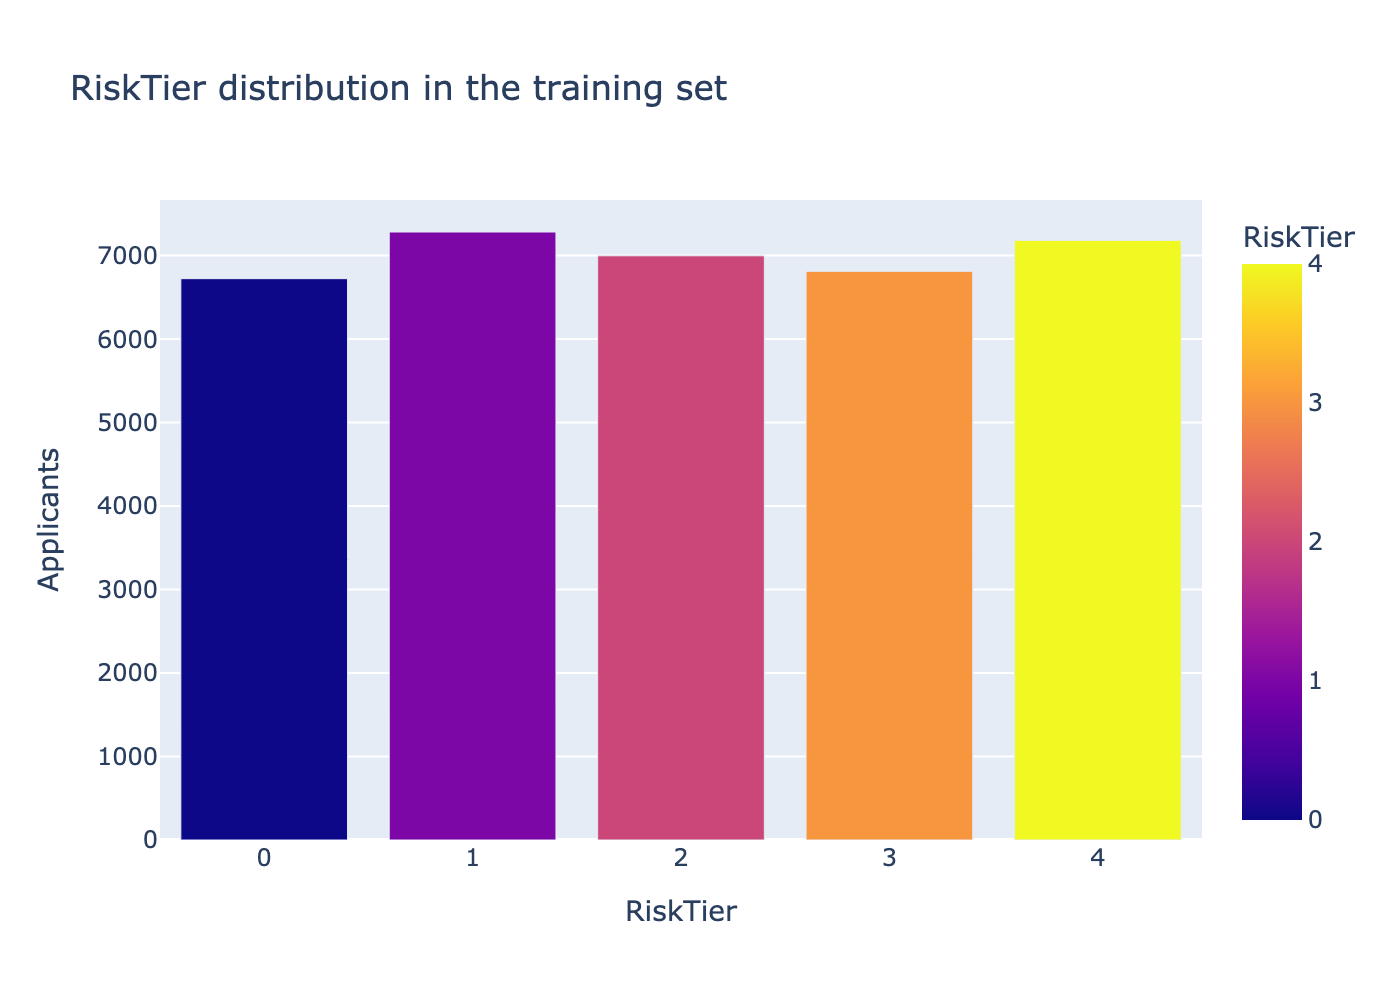
\includegraphics[width=\linewidth]{figures/class_distribution.png}
        \caption{Risk tiers are reasonably balanced.}
    \end{subfigure}
    \hfill
    \begin{subfigure}[t]{0.48\linewidth}
        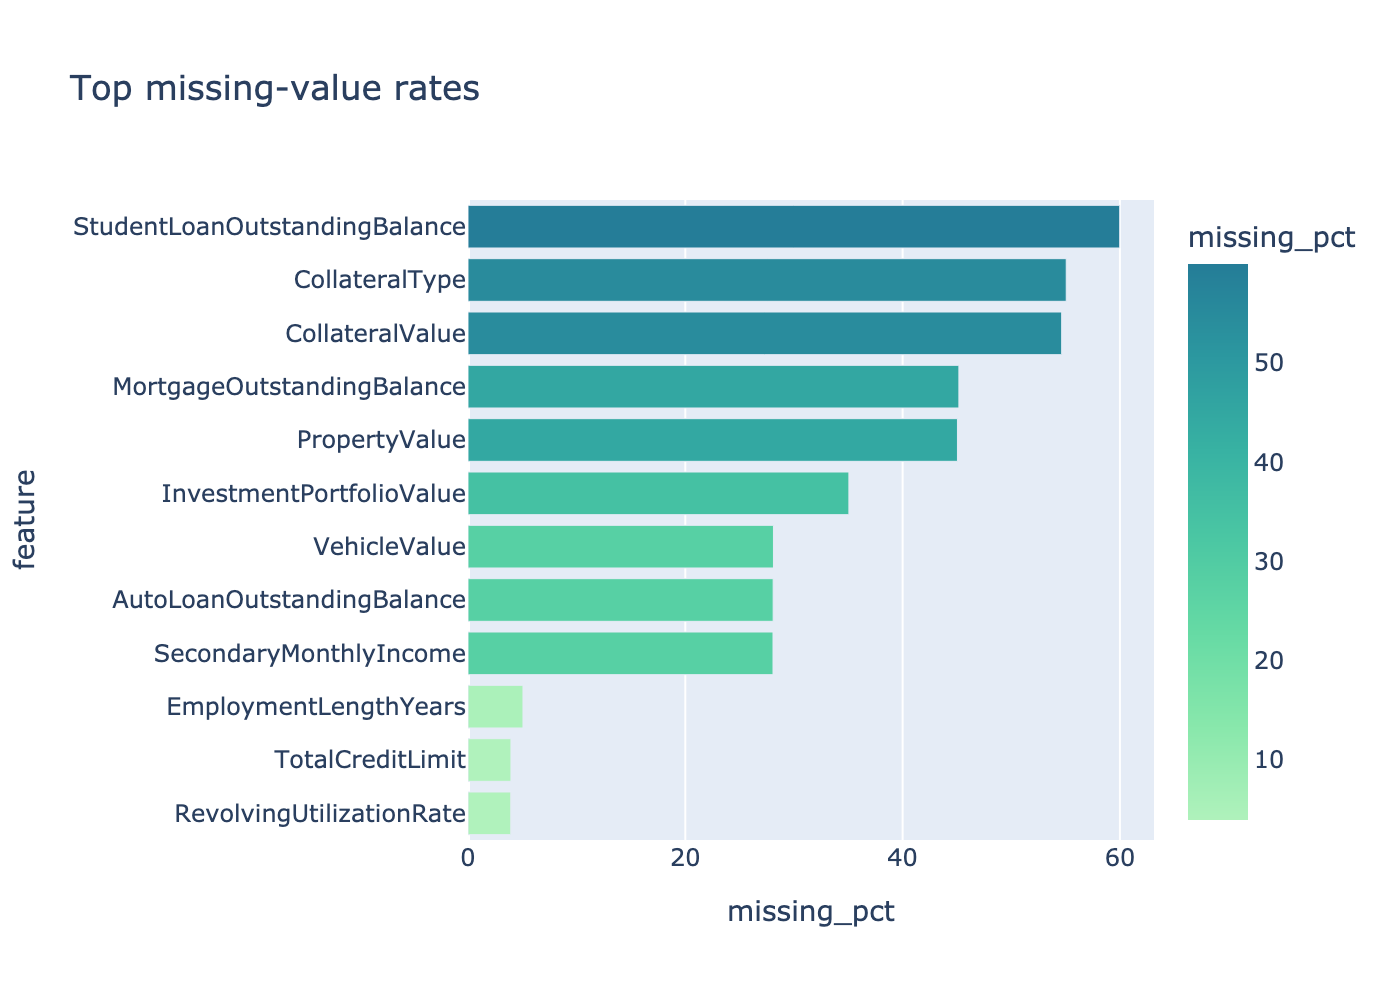
\includegraphics[width=\linewidth]{figures/missingness_overview.png}
        \caption{Missingness is concentrated in meaningful financial columns.}
    \end{subfigure}
    \caption{The early data check was reassuring in one way and tricky in another: class balance was fine, but missing values clearly carried signal.}
    \label{fig:eda-summary}
\end{figure}

That point becomes clearer once the missing columns are conditioned on context. In Figure~\ref{fig:context-corr}, \texttt{PropertyValue} and \texttt{MortgageOutstandingBalance} are missing for about 80\% of renters and applicants living with family, but only for about 16--17\% of owners or mortgage holders. Student-loan balances show a similar pattern by age: they are absent for the entire oldest age bucket and present much more often for younger borrowers. We therefore treated missingness as a feature to explain, not noise to erase.

\begin{figure}[H]
    \centering
    \begin{subfigure}[t]{0.48\linewidth}
        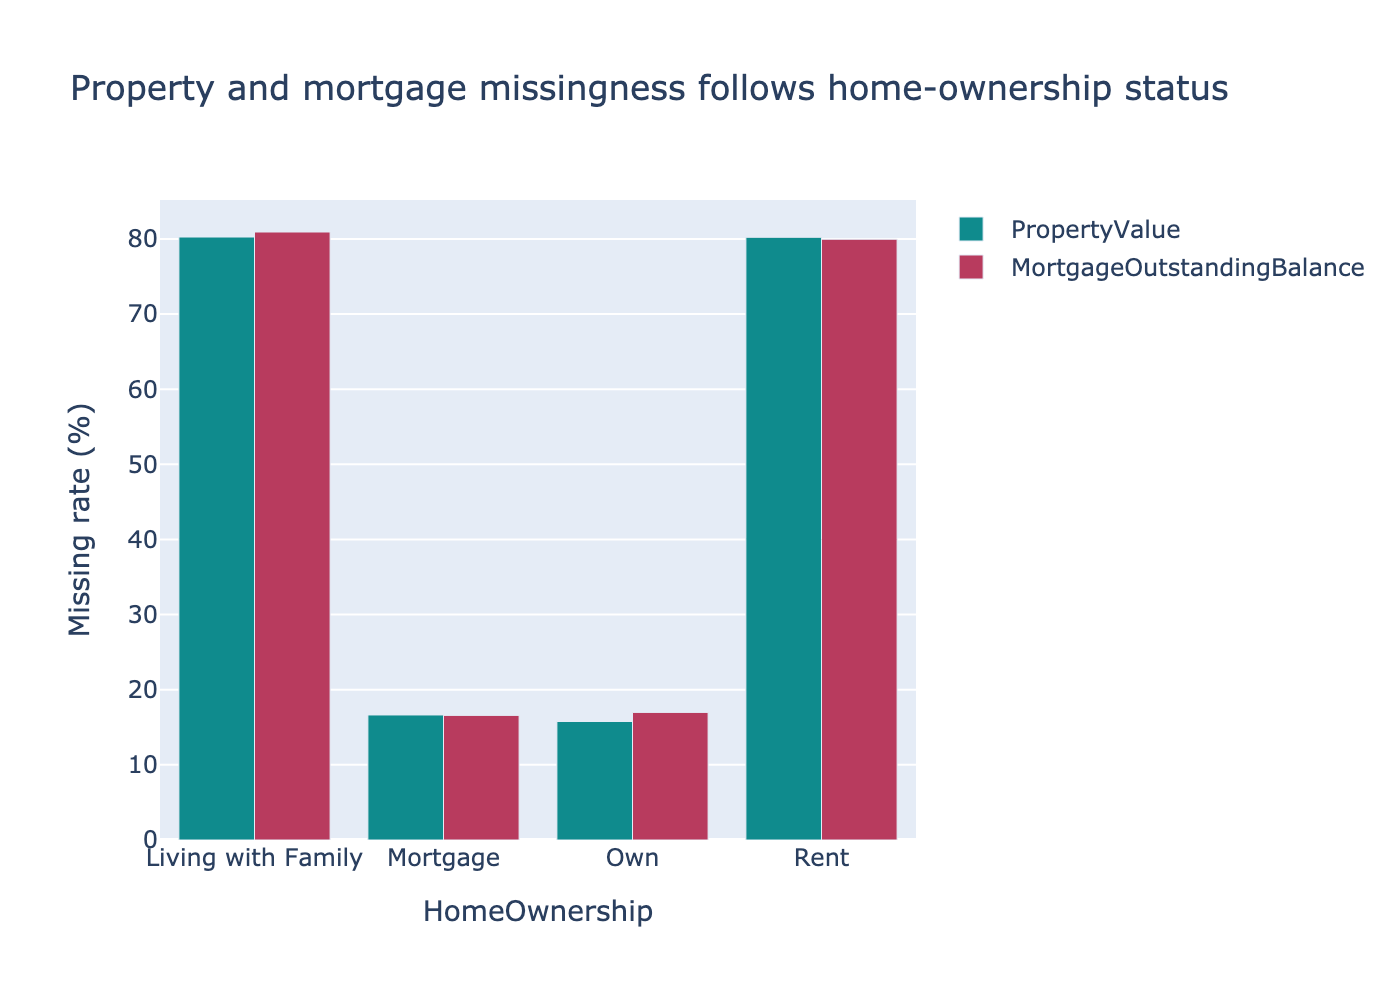
\includegraphics[width=\linewidth]{figures/semantic_missingness_context.png}
        \caption{Property and mortgage blanks are tightly linked to home-ownership status.}
    \end{subfigure}
    \hfill
    \begin{subfigure}[t]{0.48\linewidth}
        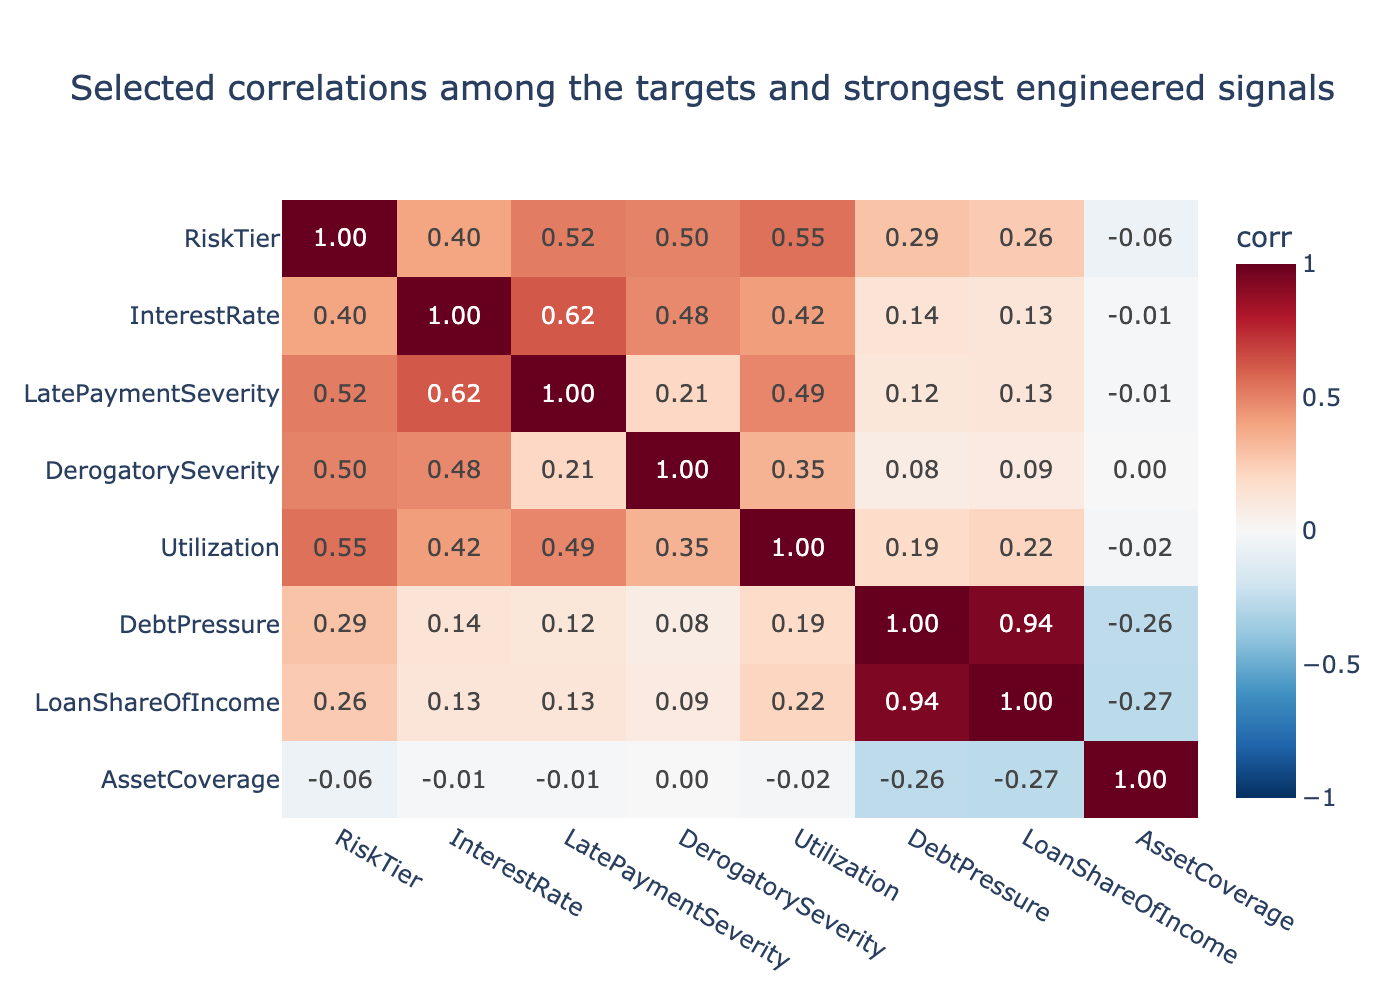
\includegraphics[width=\linewidth]{figures/correlation_focus.png}
        \caption{Delinquency and utilization features align most strongly with both targets.}
    \end{subfigure}
    \caption{Two findings shaped the rest of the pipeline: missing values were contextual, and the strongest raw relationships were concentrated in delinquency and utilization signals.}
    \label{fig:context-corr}
\end{figure}

The second useful observation was that the two targets overlap, but not perfectly. The mean offered APR rises from 6.01\% in tier 0 to 11.55\% in tier 4, yet there is still visible overlap across the lower four classes. This is why the regression problem could not simply be treated as a deterministic mapping from the class label. The correlation heatmap in Figure~\ref{fig:context-corr} makes the same point from another angle: \texttt{RevolvingUtilizationRate}, \texttt{LatePaymentSeverity}, and \texttt{DerogatorySeverity} correlate most strongly with both targets, while affordability and coverage features are weaker but still complementary.

Preprocessing was intentionally conservative:
\begin{itemize}
    \item numeric columns were median-filled only after explicit missingness indicators were created;
    \item categorical columns were preserved as strings for CatBoost, while the shared matrix used stable ordinal encoding and simple frequency features;
    \item no resampling was applied because the class histogram was already balanced enough;
    \item one fixed stratified split with seed 42 was reused for branch comparison and feature screening.
\end{itemize}

These choices kept the raw borrower structure intact. In particular, the preprocessing stage did not try to smooth away financial asymmetries that later became useful engineered features.
